
%(BEGIN_QUESTION)
% Copyright 2011, Tony R. Kuphaldt, released under the Creative Commons Attribution License (v 1.0)
% This means you may do almost anything with this work of mine, so long as you give me proper credit

A radio transmitter connects to an antenna through a coaxial cable.  The power output of the transmitter (measured at the beginning of the cable) is 2.5 watts.  The antenna only receives 2.1 watts (measured at the end of the cable, where the antenna connects).  Calculate the loss of the cable in dB per foot, given a cable length of 20 feet:

$$\includegraphics[width=15.5cm]{i02456x01.eps}$$

$L_{cable}$ = \underbar{\hskip 50pt} dB per foot

\underbar{file i02456}
%(END_QUESTION)





%(BEGIN_ANSWER)

$L_{cable}$ = \underbar{\bf 0.03786} dB per foot

\vskip 10pt

Note: either a positive or a negative value will be accepted as the answer.

%(END_ANSWER)





%(BEGIN_NOTES)

{\bf This question is intended for exams only and not worksheets!}.

%(END_NOTES)


